\chapter{OCL (Object Constraint Language)}
In questo capitolo viene utilizzato il linguaggio Object Constraint Language (OCL) per descrivere formalmente dei vincoli necessari al corretto funzionamento del sistema. Questo linguaggio è utilizzato perchè non ci sono altri modi per descrivere tali limitazioni nel contesto UML.

\section{Verifica credenziali}

Per permettere all'amministratore di effettuare il login è necessario che esso non lo abbia già effettuato. L'attributo \texttt{autenticato} nella classe \texttt{Autenticatore} deve quindi essere impostato a \texttt{false} prima della chiamata della funzione. Viene proposta questa condizione mediante precondizione in OCL:

\begin{figure}[ht]
    \centering
    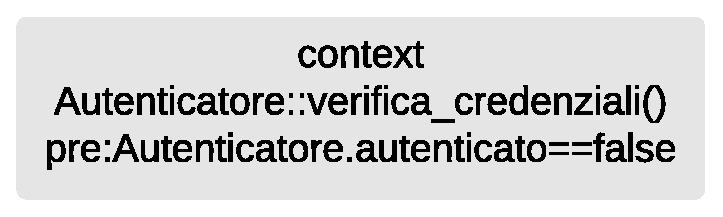
\includegraphics[scale=0.5]{Img/OCLAutenticatore.eps}
\end{figure}

\section{Effettua logout}

L'amministratore che desidera effettuare il logout deve necessariamente aver effettuato il login, inoltre dopo aver effettuato il logout esso deve essere in grado di effettuare nuovamente il login. Di seguito viene espresso mediante OCL utilizzando una pre-condizione ed una post-condizione.

\begin{figure}[ht]
    \centering
    \includegraphics[scale=0.5]{Img/OCLVisualizzatoreMenù.eps}
\end{figure}

\section{Generazione istogramma}

Per poter generare l'istogramma è necessario che il lasso temporale selezionato esista, ossia che l'attributo inizio abbia un valore minore di fine. Essendo  \texttt{Tempo} un valore non primitivo bisogna confrontare nel seguente ordine anno, mese, giorno, ore, minuti e secondi nel caso anche i minuti avessero lo stesso valore.

Un'altra condizione necessaria per richiedere la generazione dell'istogramma è che l'utente sia autenticato, ossia che l'attributo \texttt{autenticato} nella classe \texttt{Autenticatore} sia impostato a \texttt{True}.

I seguenti due vincoli sono espressi mediante OCL utilizzando un'invariante e una precondizione con il seguente codice:

\begin{figure}[ht]
    \centering
    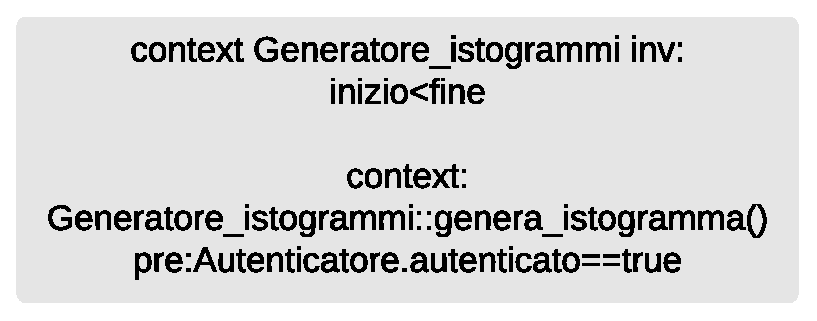
\includegraphics[scale=0.5]{Img/OCLGeneratoreIstogrammi.eps}
\end{figure}